\section{Our Approach}

\begin{figure*}[t]
    \centering
    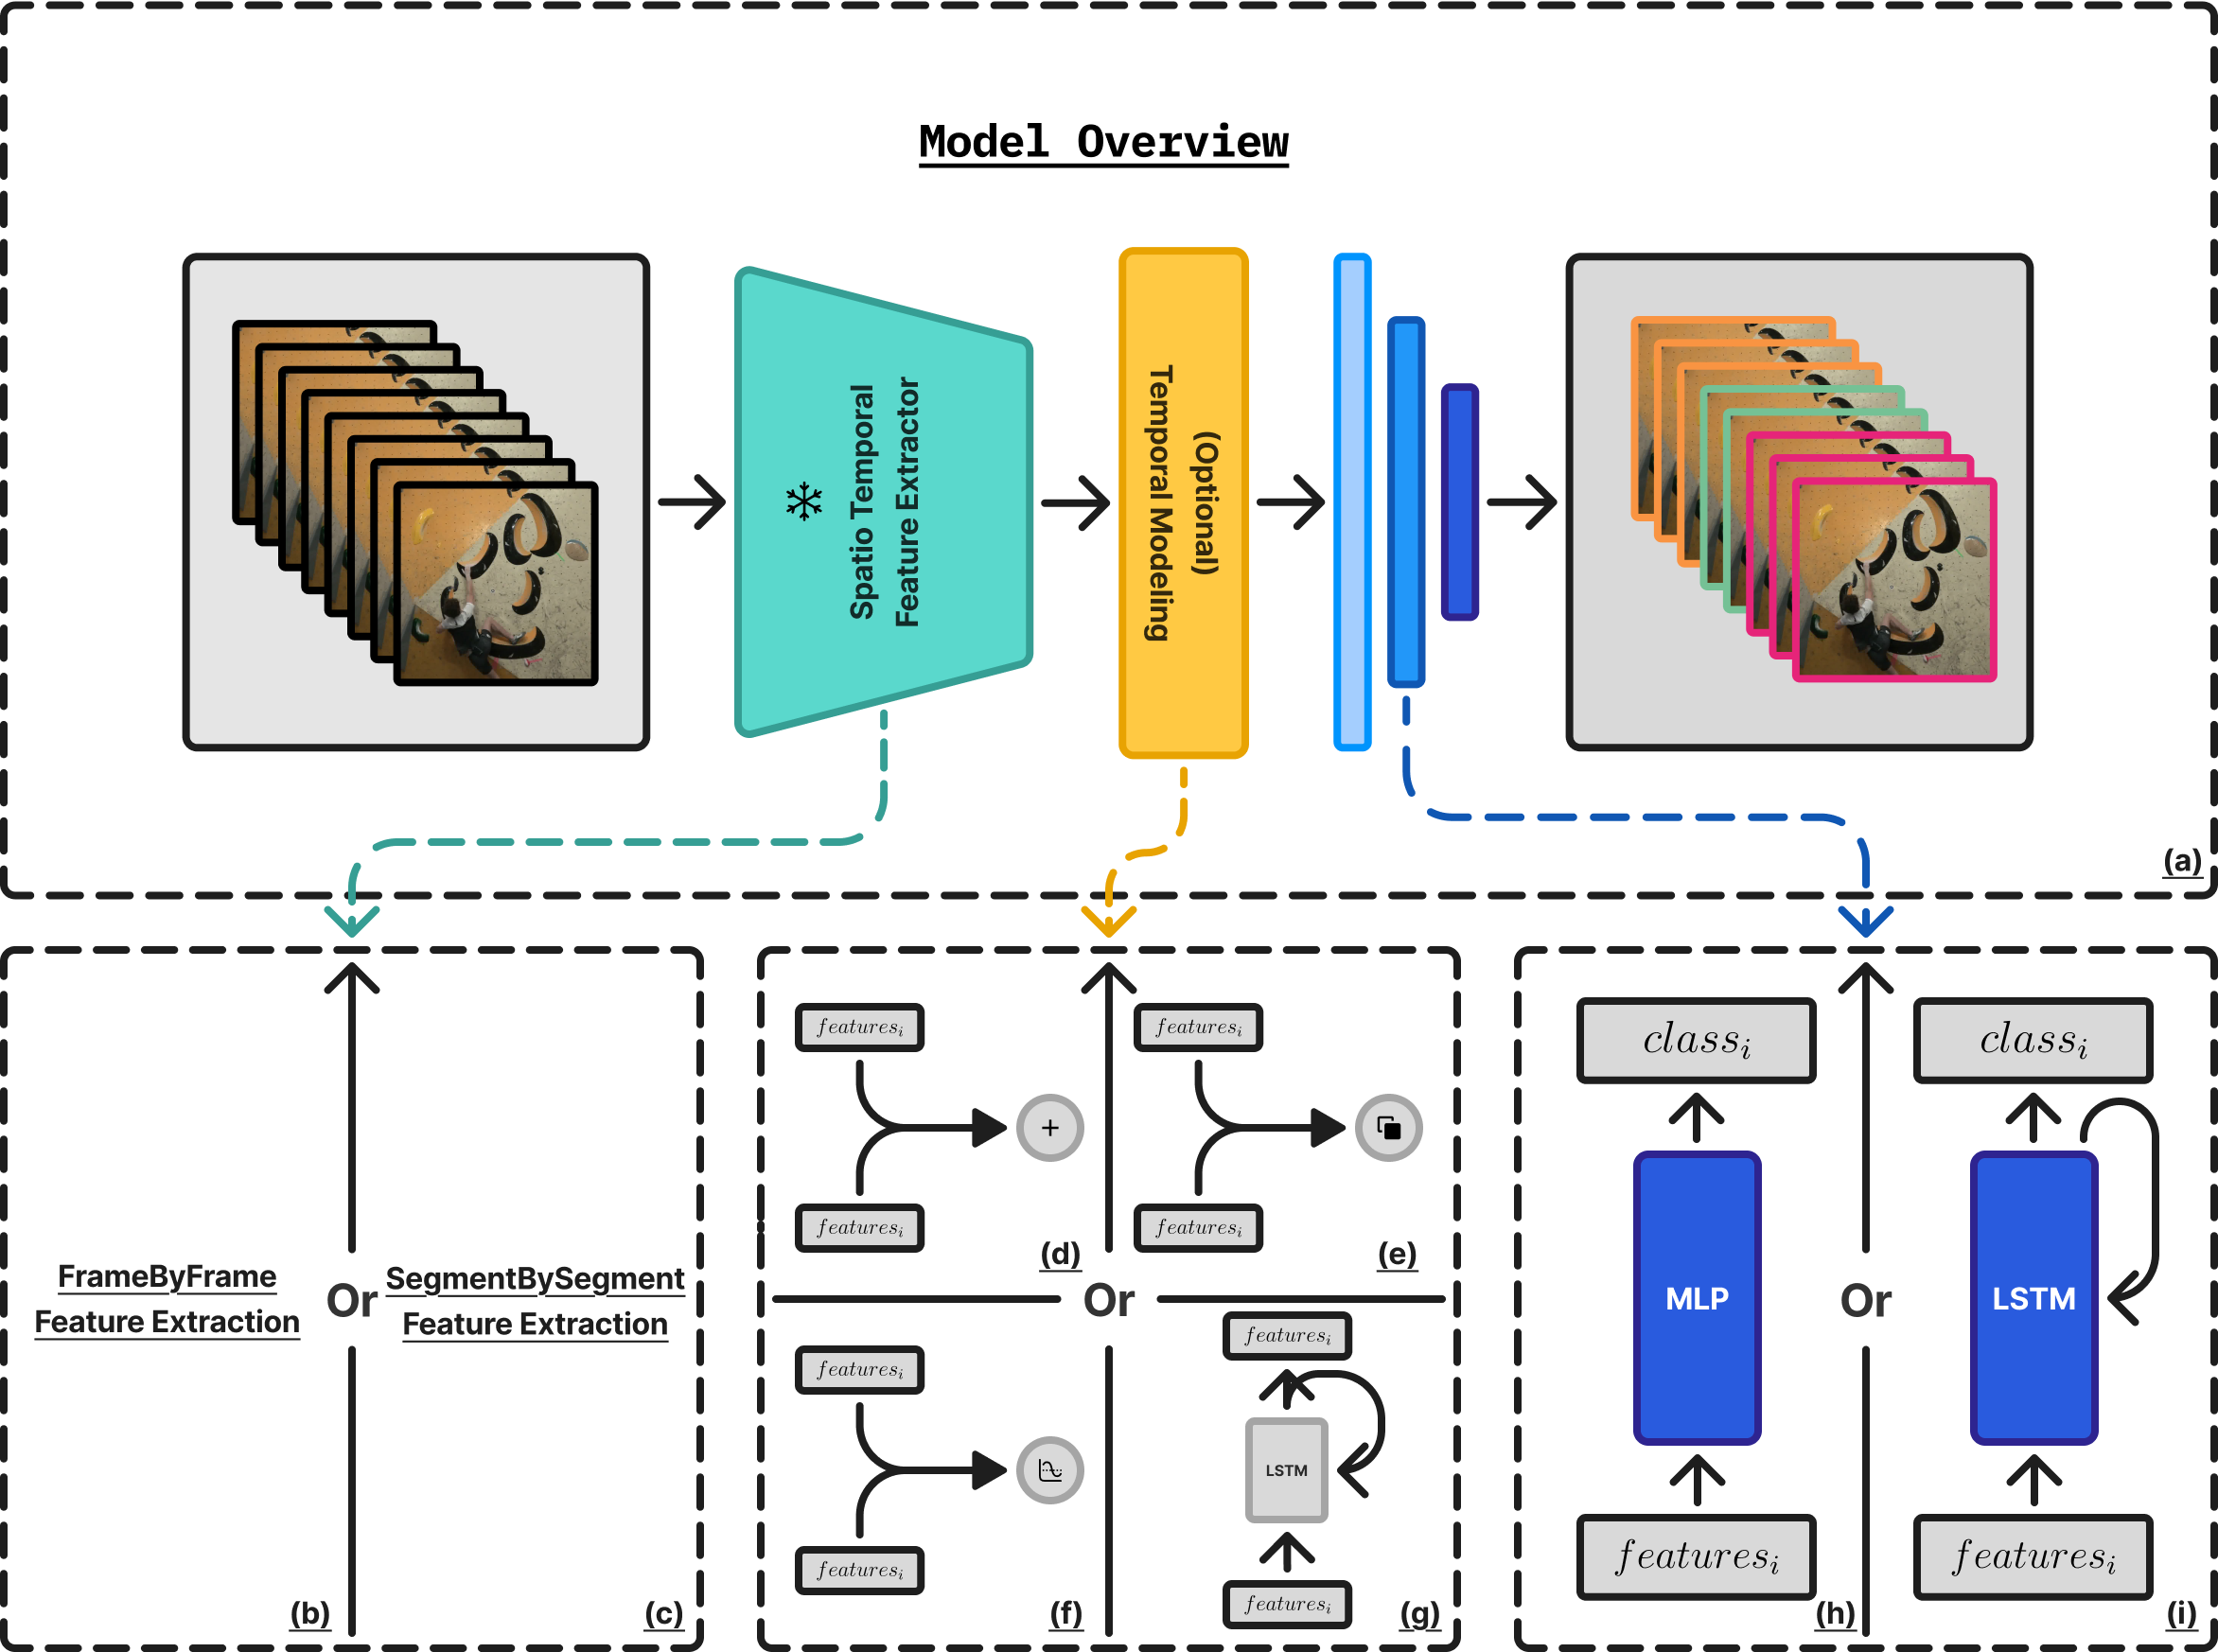
\includegraphics[width=\textwidth]{../../assets/figures/model-overview.png}
    \caption{Model Architecture Overview.}
    \label{figure:model-architecture-overview}
    \medskip
    \small\par
    % \small
    (a) Represent a global overview of our Model's architecture. (b) and (c) represent the types of spatio temporal feature extractors considered. (d), (e), (f) and (g) represent the different ways of aggregating the frame by frame feature into a single feature representing a sequence of frames. (h) and (i) represent the two architectures of feature classifiers we considered, and MLP and an LSTM respectively.
\end{figure*}

Given the dataset size constraint, training a neural network from scratch with our data is infeasible and unlikely to yield meaningful results. To address this, we leverage pre-trained networks trained on large-scale datasets that contain similar types of actions to those found in our data. These actions are general, composed of multiple smaller movements, and not very detailed, making them comparable to activities present in popular datasets like Kinetics.

Our strategy involves utilizing these pre-trained networks to extract feature representations from our videos, clips, and frames. Specifically, we extract features from the hidden layers of these networks — typically the layer immediately preceding the final classification layer — as they encode rich spatio-temporal information relevant to our task. These extracted features are then fed into a custom network designed for classification on our custom action labels.

This approach addresses multiple constraints simultaneously. First, it mitigates the impact of our limited dataset by capitalizing on robust features learned from extensive pre-training. Second, it reduces the computational burden, as we avoid the costly process of training a deep network from scratch. Finally, this method is well-suited to our project timeline, as designing and training a complex architecture would exceed our allocated 120 hours for this research project.

In the following sections, we describe the key components of our approach described in Figure~\ref{figure:model-architecture-overview} and how we train it.

\subsection{Spatio-Temporal Feature Extractors}
The backbone of our model is a spatio-temporal feature extractor designed to capture both spatial and temporal information from video data. We employ pre-trained models for this component, freezing their weights to retain the learned representations.

Two types of models are explored for this purpose: frame-level feature extractors and segment-level feature extractors.

\subsubsection{Frame-Level Extractors}
Frame-level extractors process individual frames independently to extract spatial features. Examples include 2D CNNs such as \modelname{ResNet}, vision transformers like \modelname{DINO}, \modelname{CLIP}, or \modelname{ViT}, and potentially pseudo handcrafted features such as object presence (e.g., brushes) and / or positional key points.

While (pseudo) handcrafted features can be interpretable and informative, they introduce biases and require additional training for object detection — to detect the presence and position of a brush for example — which is resource-intensive. Thus, our approach prioritizes automated feature extractors to maximize efficiency and robustness.

Once frame-level features are extracted, we explore several strategies to aggregate these features into a single representation for each video segment:

\noindent\textbf{\small{Averaging.}} The most common method, recommended in the literature \cite{dinov2} for its simplicity and effectiveness.
\noindent\textbf{\small{Addition.}} Similar to averaging but involves summing the features directly. 
\noindent\textbf{\small{Concatenation.}} Combines frame features without any additional operations. According to \cite{dinov2}, this method is the most effective in capturing temporal information \& thus it is the one we opted to use.
\noindent\textbf{\small{Temporal Modeling.}} Uses models like LSTMs or Transformers to capture temporal dependencies, offering improved contextual understanding at the cost of higher computational complexity. \cite{action-clip}.

\subsubsection{Segment-Level Extractors}
Segment-level extractors process multiple consecutive frames directly, capturing both spatial and temporal patterns. Examples include 3D CNNs, which extend 2D CNN architectures to model motion and temporal dynamics, and transformer-based models that have demonstrated strong performance on video tasks. While effective, these models are typically more computationally demanding.

A list of all the spatio-temporal feature extractors we considered can be found in the Appendix.

\subsection{Temporal Context Window}
The temporal context window defines the number of consecutive frames the model processes at once. Choosing an optimal window size is crucial:

\noindent\textbf{\small{Short Window.}}
It may not capture sufficient context for accurate classification.

\noindent\textbf{\small{Long Window.}}
It risks embedding the entire video into a single feature, increasing computational costs and reducing model flexibility.

As the temporal context window of the backbone networks is quite limited to around 16-32 frames usually, processing the whole 4 minutes of video and extracting a single feature for the entire video is both computationally costly and not practical in our case. This would be more practical for video classification tasks, where the goal is to classify the whole video. In our case, we aim to extract different time segments and classify them individually.

\subsection{Temporal Sub-Sampling}
To improve efficiency without sacrificing performance, we incorporate temporal sub-sampling. This technique involves reducing the frame rate before feature extraction, as consecutive frames in bouldering videos often exhibit minimal visual change. Temporal sub-sampling is a simple yet highly effective method for reducing computational load without significant performance degradation \cite{impact-of-temporal-subsampling}.

By combining pre-trained feature extractors, temporal sub-sampling, and thoughtful hyperparameter tuning, our approach aims to achieve robust performance despite dataset limitations.

\subsection{Classifier Model}

For classification, we consider two different model architectures: a Multi-Layer Perceptron (MLP) and a Long Short-Term Memory (LSTM) network. Both approaches are designed to process the spatio-temporal features extracted from the pre-trained models.

\noindent\textbf{MLP Approach.} The MLP used in our approach consists of a simple linear layer with no activation function and a bias term. This architecture has been shown to yield the best performance in our case, as more complex network structures tend to overfit the limited training data. The simplicity of the MLP helps avoid overfitting while maintaining efficiency, making it ideal for our constraints. The output of this linear layer is fed directly into the softmax function to produce class probabilities for the classification task.

\noindent\textbf{LSTM Approach.} The LSTM used in our approach consists of a single LSTM layer with a hidden state size of 128. This configuration enables the model to capture temporal dependencies between frames or video segments, which is critical for action recognition tasks where context across time is crucial. The LSTM’s output is passed through a linear layer (similar to the MLP) to predict the class for each segment.

Both models were validated using cross-validation to identify the most effective hyperparameters for our dataset.

%  --- --- ---

\subsection{Training Methodology}

\subsubsection*{Backbone Model}
We experimented with several backbone models for feature extraction, leveraging both frame-level and segment-level networks. Notable examples include:

\modelname{DINO} and \modelname{CLIP.} Vision Transformers used as frame-level feature extractors for their strong spatial representation capabilities.

\modelname{X3D}, \modelname{R3D}, and \modelname{Slowfast.} Segment-level extractors known for their robust spatio-temporal modeling.

Most of the backbones we use are pre-trained or fine-tuned on the Kinetics dataset, except for \modelname{CLIP}, which leverages large-scale internet data.

\subsubsection*{Loss Function}
Our classification model is trained using the \textbf{cross-entropy loss} function, defined as:

\[
\mathcal{L} = -\sum_{i=1}^{N} y_i \log \hat{y}_i
\]

where \(y_i\) is the true label and \(\hat{y}_i\) is the predicted probability for class \(i\). While cross-entropy loss effectively handles multi-class classification, alternative losses such as focal loss or label-smoothing loss have been proposed in the literature to address class imbalance and calibration issues. These approaches may be worth exploring in future work.

\subsubsection*{Training Setup}

To prevent data leakage during validation, we ensured that segments from the same video were never split across training and validation sets. This avoids the model unintentionally learning video-specific patterns rather than generalizable features.

\subsubsection*{Data Filtering and Preprocessing}
To improve data quality and enhance model performance, we applied several preprocessing steps:

\noindent\textbf{Removal of Personless Frames.} Frames without visible climbers were excluded to reduce noise. This was done by detecting the presence of a person in each frame using a pre-trained object detection model (\modelname{YOLO}) \cite{yolo}.

\noindent\textbf{Cleaning of Low-Quality Data.} Unannotated frames were removed rather than assigning them a generic "nothing" label. This improved class balance and reduced label ambiguity.

\noindent\textbf{Stopwatch Class Removal.} We removed segments with the stopwatch class, as they were highly imbalanced and lacked distinction. Climbers often exit the frame while checking the timer, and it varies across competitions, making it inconsistent in our dataset.

\begin{AIbox}{Python Package - Cached Dataset.}
    To accelerate training, we developed a custom Python package called \textbf{cached-dataset} - \href{https://github.com/raideno/cached-dataset}{https://github.com/raideno/cached-dataset}. This tool caches the transformation of a dataset to disk, significantly reducing data loading overhead during training and feature extraction. This allow us to efficiently iterate through training experiments and hyperparameter tuning.
\end{AIbox}

By combining robust pre-trained feature extractors, temporal sub-sampling, and thoughtful data filtering strategies, our training methodology effectively addresses the challenges posed by our limited dataset. These strategies ensured a stable and efficient training process while maximizing model performance.